% Options for packages loaded elsewhere
\PassOptionsToPackage{unicode}{hyperref}
\PassOptionsToPackage{hyphens}{url}
\PassOptionsToPackage{dvipsnames,svgnames,x11names}{xcolor}
%
\documentclass[
  letterpaper,
  DIV=11,
  numbers=noendperiod]{scrartcl}

\usepackage{amsmath,amssymb}
\usepackage{iftex}
\ifPDFTeX
  \usepackage[T1]{fontenc}
  \usepackage[utf8]{inputenc}
  \usepackage{textcomp} % provide euro and other symbols
\else % if luatex or xetex
  \usepackage{unicode-math}
  \defaultfontfeatures{Scale=MatchLowercase}
  \defaultfontfeatures[\rmfamily]{Ligatures=TeX,Scale=1}
\fi
\usepackage{lmodern}
\ifPDFTeX\else  
    % xetex/luatex font selection
\fi
% Use upquote if available, for straight quotes in verbatim environments
\IfFileExists{upquote.sty}{\usepackage{upquote}}{}
\IfFileExists{microtype.sty}{% use microtype if available
  \usepackage[]{microtype}
  \UseMicrotypeSet[protrusion]{basicmath} % disable protrusion for tt fonts
}{}
\makeatletter
\@ifundefined{KOMAClassName}{% if non-KOMA class
  \IfFileExists{parskip.sty}{%
    \usepackage{parskip}
  }{% else
    \setlength{\parindent}{0pt}
    \setlength{\parskip}{6pt plus 2pt minus 1pt}}
}{% if KOMA class
  \KOMAoptions{parskip=half}}
\makeatother
\usepackage{xcolor}
\setlength{\emergencystretch}{3em} % prevent overfull lines
\setcounter{secnumdepth}{-\maxdimen} % remove section numbering
% Make \paragraph and \subparagraph free-standing
\makeatletter
\ifx\paragraph\undefined\else
  \let\oldparagraph\paragraph
  \renewcommand{\paragraph}{
    \@ifstar
      \xxxParagraphStar
      \xxxParagraphNoStar
  }
  \newcommand{\xxxParagraphStar}[1]{\oldparagraph*{#1}\mbox{}}
  \newcommand{\xxxParagraphNoStar}[1]{\oldparagraph{#1}\mbox{}}
\fi
\ifx\subparagraph\undefined\else
  \let\oldsubparagraph\subparagraph
  \renewcommand{\subparagraph}{
    \@ifstar
      \xxxSubParagraphStar
      \xxxSubParagraphNoStar
  }
  \newcommand{\xxxSubParagraphStar}[1]{\oldsubparagraph*{#1}\mbox{}}
  \newcommand{\xxxSubParagraphNoStar}[1]{\oldsubparagraph{#1}\mbox{}}
\fi
\makeatother

\usepackage{color}
\usepackage{fancyvrb}
\newcommand{\VerbBar}{|}
\newcommand{\VERB}{\Verb[commandchars=\\\{\}]}
\DefineVerbatimEnvironment{Highlighting}{Verbatim}{commandchars=\\\{\}}
% Add ',fontsize=\small' for more characters per line
\usepackage{framed}
\definecolor{shadecolor}{RGB}{241,243,245}
\newenvironment{Shaded}{\begin{snugshade}}{\end{snugshade}}
\newcommand{\AlertTok}[1]{\textcolor[rgb]{0.68,0.00,0.00}{#1}}
\newcommand{\AnnotationTok}[1]{\textcolor[rgb]{0.37,0.37,0.37}{#1}}
\newcommand{\AttributeTok}[1]{\textcolor[rgb]{0.40,0.45,0.13}{#1}}
\newcommand{\BaseNTok}[1]{\textcolor[rgb]{0.68,0.00,0.00}{#1}}
\newcommand{\BuiltInTok}[1]{\textcolor[rgb]{0.00,0.23,0.31}{#1}}
\newcommand{\CharTok}[1]{\textcolor[rgb]{0.13,0.47,0.30}{#1}}
\newcommand{\CommentTok}[1]{\textcolor[rgb]{0.37,0.37,0.37}{#1}}
\newcommand{\CommentVarTok}[1]{\textcolor[rgb]{0.37,0.37,0.37}{\textit{#1}}}
\newcommand{\ConstantTok}[1]{\textcolor[rgb]{0.56,0.35,0.01}{#1}}
\newcommand{\ControlFlowTok}[1]{\textcolor[rgb]{0.00,0.23,0.31}{\textbf{#1}}}
\newcommand{\DataTypeTok}[1]{\textcolor[rgb]{0.68,0.00,0.00}{#1}}
\newcommand{\DecValTok}[1]{\textcolor[rgb]{0.68,0.00,0.00}{#1}}
\newcommand{\DocumentationTok}[1]{\textcolor[rgb]{0.37,0.37,0.37}{\textit{#1}}}
\newcommand{\ErrorTok}[1]{\textcolor[rgb]{0.68,0.00,0.00}{#1}}
\newcommand{\ExtensionTok}[1]{\textcolor[rgb]{0.00,0.23,0.31}{#1}}
\newcommand{\FloatTok}[1]{\textcolor[rgb]{0.68,0.00,0.00}{#1}}
\newcommand{\FunctionTok}[1]{\textcolor[rgb]{0.28,0.35,0.67}{#1}}
\newcommand{\ImportTok}[1]{\textcolor[rgb]{0.00,0.46,0.62}{#1}}
\newcommand{\InformationTok}[1]{\textcolor[rgb]{0.37,0.37,0.37}{#1}}
\newcommand{\KeywordTok}[1]{\textcolor[rgb]{0.00,0.23,0.31}{\textbf{#1}}}
\newcommand{\NormalTok}[1]{\textcolor[rgb]{0.00,0.23,0.31}{#1}}
\newcommand{\OperatorTok}[1]{\textcolor[rgb]{0.37,0.37,0.37}{#1}}
\newcommand{\OtherTok}[1]{\textcolor[rgb]{0.00,0.23,0.31}{#1}}
\newcommand{\PreprocessorTok}[1]{\textcolor[rgb]{0.68,0.00,0.00}{#1}}
\newcommand{\RegionMarkerTok}[1]{\textcolor[rgb]{0.00,0.23,0.31}{#1}}
\newcommand{\SpecialCharTok}[1]{\textcolor[rgb]{0.37,0.37,0.37}{#1}}
\newcommand{\SpecialStringTok}[1]{\textcolor[rgb]{0.13,0.47,0.30}{#1}}
\newcommand{\StringTok}[1]{\textcolor[rgb]{0.13,0.47,0.30}{#1}}
\newcommand{\VariableTok}[1]{\textcolor[rgb]{0.07,0.07,0.07}{#1}}
\newcommand{\VerbatimStringTok}[1]{\textcolor[rgb]{0.13,0.47,0.30}{#1}}
\newcommand{\WarningTok}[1]{\textcolor[rgb]{0.37,0.37,0.37}{\textit{#1}}}

\providecommand{\tightlist}{%
  \setlength{\itemsep}{0pt}\setlength{\parskip}{0pt}}\usepackage{longtable,booktabs,array}
\usepackage{calc} % for calculating minipage widths
% Correct order of tables after \paragraph or \subparagraph
\usepackage{etoolbox}
\makeatletter
\patchcmd\longtable{\par}{\if@noskipsec\mbox{}\fi\par}{}{}
\makeatother
% Allow footnotes in longtable head/foot
\IfFileExists{footnotehyper.sty}{\usepackage{footnotehyper}}{\usepackage{footnote}}
\makesavenoteenv{longtable}
\usepackage{graphicx}
\makeatletter
\newsavebox\pandoc@box
\newcommand*\pandocbounded[1]{% scales image to fit in text height/width
  \sbox\pandoc@box{#1}%
  \Gscale@div\@tempa{\textheight}{\dimexpr\ht\pandoc@box+\dp\pandoc@box\relax}%
  \Gscale@div\@tempb{\linewidth}{\wd\pandoc@box}%
  \ifdim\@tempb\p@<\@tempa\p@\let\@tempa\@tempb\fi% select the smaller of both
  \ifdim\@tempa\p@<\p@\scalebox{\@tempa}{\usebox\pandoc@box}%
  \else\usebox{\pandoc@box}%
  \fi%
}
% Set default figure placement to htbp
\def\fps@figure{htbp}
\makeatother

\KOMAoption{captions}{tableheading}
\usepackage{float}
\floatplacement{table}{H}
\floatplacement{figure}{H}
\makeatletter
\@ifpackageloaded{caption}{}{\usepackage{caption}}
\AtBeginDocument{%
\ifdefined\contentsname
  \renewcommand*\contentsname{Tabla de contenidos}
\else
  \newcommand\contentsname{Tabla de contenidos}
\fi
\ifdefined\listfigurename
  \renewcommand*\listfigurename{Listado de Figuras}
\else
  \newcommand\listfigurename{Listado de Figuras}
\fi
\ifdefined\listtablename
  \renewcommand*\listtablename{Listado de Tablas}
\else
  \newcommand\listtablename{Listado de Tablas}
\fi
\ifdefined\figurename
  \renewcommand*\figurename{Figura}
\else
  \newcommand\figurename{Figura}
\fi
\ifdefined\tablename
  \renewcommand*\tablename{Tabla}
\else
  \newcommand\tablename{Tabla}
\fi
}
\@ifpackageloaded{float}{}{\usepackage{float}}
\floatstyle{ruled}
\@ifundefined{c@chapter}{\newfloat{codelisting}{h}{lop}}{\newfloat{codelisting}{h}{lop}[chapter]}
\floatname{codelisting}{Listado}
\newcommand*\listoflistings{\listof{codelisting}{Listado de Listados}}
\makeatother
\makeatletter
\makeatother
\makeatletter
\@ifpackageloaded{caption}{}{\usepackage{caption}}
\@ifpackageloaded{subcaption}{}{\usepackage{subcaption}}
\makeatother
\makeatletter
\@ifpackageloaded{tikz}{}{\usepackage{tikz}}
\makeatother
        \newcommand*\circled[1]{\tikz[baseline=(char.base)]{
          \node[shape=circle,draw,inner sep=1pt] (char) {{\scriptsize#1}};}}  
                  

\ifLuaTeX
\usepackage[bidi=basic]{babel}
\else
\usepackage[bidi=default]{babel}
\fi
\babelprovide[main,import]{spanish}
% get rid of language-specific shorthands (see #6817):
\let\LanguageShortHands\languageshorthands
\def\languageshorthands#1{}
\usepackage{bookmark}

\IfFileExists{xurl.sty}{\usepackage{xurl}}{} % add URL line breaks if available
\urlstyle{same} % disable monospaced font for URLs
\hypersetup{
  pdftitle={Quarto Markdown Básico: Parte 2 (figuras)},
  pdflang={es},
  colorlinks=true,
  linkcolor={blue},
  filecolor={Maroon},
  citecolor={Blue},
  urlcolor={Blue},
  pdfcreator={LaTeX via pandoc}}


\title{Quarto Markdown Básico: Parte 2 (figuras)}
\author{}
\date{}

\begin{document}
\maketitle

\renewcommand*\contentsname{Tabla de contenidos}
{
\hypersetup{linkcolor=}
\setcounter{tocdepth}{3}
\tableofcontents
}

\section{Imágenes}\label{imuxe1genes}

Algunas referencias interesantes sobre figuras o imágenes en Quarto:

\begin{itemize}
\tightlist
\item
  \url{https://quarto.org/docs/authoring/figures.html}
\end{itemize}

La cabecera yaml de este documento es:

\phantomsection\label{annotated-cell-1}%
\begin{Shaded}
\begin{Highlighting}[]
\PreprocessorTok{{-}{-}{-}}
\FunctionTok{title}\KeywordTok{:}\AttributeTok{ }\StringTok{"Quarto Markdown Básico: Parte 2 (figuras)"}
\FunctionTok{lang}\KeywordTok{:}\AttributeTok{ es}
\FunctionTok{toc}\KeywordTok{:}\AttributeTok{ }\CharTok{true}
\FunctionTok{format}\KeywordTok{:}\AttributeTok{ }
\AttributeTok{  }\FunctionTok{html}\KeywordTok{:}
\AttributeTok{    }\FunctionTok{code{-}tools}\KeywordTok{:}\AttributeTok{ }\CharTok{true}
\AttributeTok{  }\FunctionTok{pdf}\KeywordTok{:}\AttributeTok{ }
\AttributeTok{    }\FunctionTok{keep{-}tex}\KeywordTok{:}\AttributeTok{ }\CharTok{true}\CommentTok{ }\hspace*{\fill}\NormalTok{\circled{1}}
\AttributeTok{    }\FunctionTok{header{-}includes}\KeywordTok{:}\CommentTok{ }\hspace*{\fill}\NormalTok{\circled{2}}
\AttributeTok{      }\KeywordTok{{-}}\AttributeTok{ \textbackslash{}usepackage\{float\}}\CommentTok{ }\hspace*{\fill}\NormalTok{\circled{3}}
\AttributeTok{      }\KeywordTok{{-}}\AttributeTok{ \textbackslash{}floatplacement\{table\}\{H\}}\CommentTok{ }\hspace*{\fill}\NormalTok{\circled{4}}
\AttributeTok{      }\KeywordTok{{-}}\AttributeTok{ \textbackslash{}floatplacement\{figure\}\{H\}}\CommentTok{ }\hspace*{\fill}\NormalTok{\circled{5}}
\PreprocessorTok{{-}{-}{-}}
\end{Highlighting}
\end{Shaded}

\begin{description}
\tightlist
\item[\circled{1}]
En la salida pdf, indica que el fichero LaTeX intermedio generado no se
elimine (para consultarlo).
\item[\circled{2}]
En la salida pdf, permite incluir instrucciones LaTeX en la cabecera del
fichero LaTeX (``.tex'') intermedio que se genera.
\item[\circled{3}]
Carga el paquete LaTeX: ``float''.
\item[\circled{4}]
Le indica que todas las tablas que se generan se colocarán justo en
donde se han escrito (no ``flotan'' a otros lugares).
\item[\circled{5}]
Le indica que todas las figuras que se generan se colocarán justo en
donde se han escrito (no ``flotan'' a otros lugares).
\end{description}

\subsection{Solamente la imagen}\label{solamente-la-imagen}

Escriba \texttt{!{[}{]}(img/puente.jpg)} para producir:

\pandocbounded{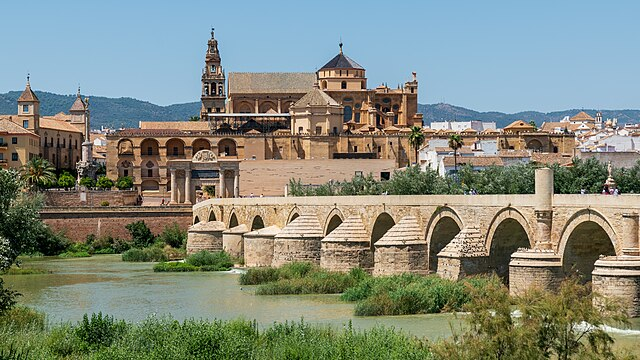
\includegraphics[keepaspectratio]{img/puente.jpg}}

\newpage{}

\subsection{Una imagen con una
descripción}\label{una-imagen-con-una-descripciuxf3n}

Escriba
\texttt{!{[}Esto\ es\ una\ foto\ de\ un\ puente{]}(img/puente.jpg)} para
producir:

\begin{figure}[H]

{\centering \pandocbounded{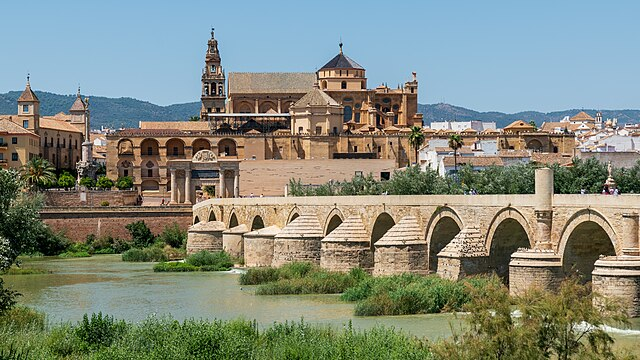
\includegraphics[keepaspectratio]{img/puente.jpg}}

}

\caption{Esto es una foto de un puente}

\end{figure}%

\newpage{}

\subsection{Una imagen con un enlace}\label{una-imagen-con-un-enlace}

Añadir corchetes y un enlace entre paréntesis como el siguiente:
\texttt{{[}!{[}Esto\ es\ una\ foto\ de\ un\ puente\ enlazada\ a\ una\ web{]}(img/puente.jpg){]}(https://es.wikipedia.org/wiki/Puente)}
para crear un imagen con un enlace como la siguiente:

\begin{figure}[H]

{\centering \pandocbounded{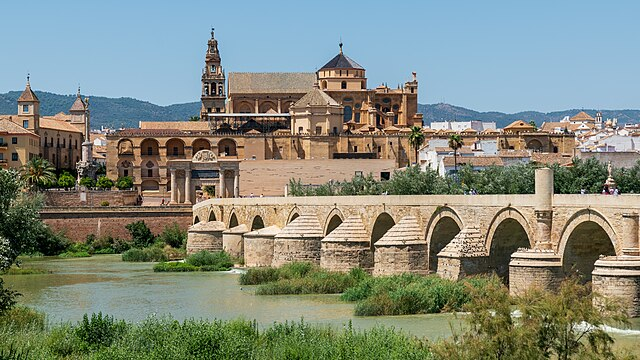
\includegraphics[keepaspectratio]{img/puente.jpg}}

}

\caption{Esto es una foto de un puente enlazada a una web}

\end{figure}%

\newpage{}

\subsection{Una imagen con una descripción en un menú emergente o
``pop-up''}\label{una-imagen-con-una-descripciuxf3n-en-un-menuxfa-emergente-o-pop-up}

Para crear un menú emergente o ``pop-up'' con una etiqueta que aparece
cuando el usuario pasa el ratón sobre la imagen, añadir un texto en
entre los paréntesis entre comillas como se muestra a continuación:
\texttt{{[}!{[}Esto\ es\ una\ foto\ de\ un\ puente\ enlazada\ con\ una\ web\ y\ con\ una\ descripción\ como\ pop-up{]}(img/puente.jpg){]}(https://es.wikipedia.org/wiki/Puente\ "Puente\ romano\ en\ Córdoba!")}
para crear una imagen como esta:

\begin{figure}[H]

{\centering \pandocbounded{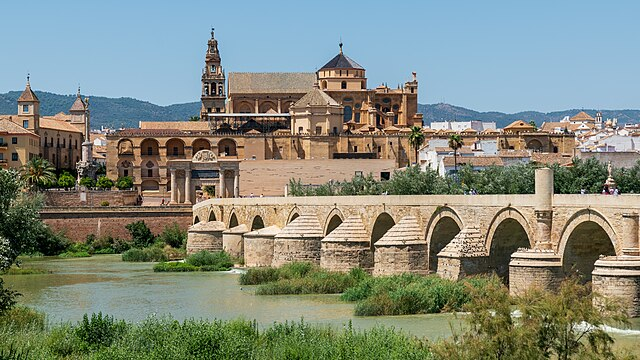
\includegraphics[keepaspectratio]{img/puente.jpg}}

}

\caption{Esto es una foto de un puente enlazada con una web y con una
descripción como pop-up}

\end{figure}%

\newpage{}

\subsection{Una imagen con un texto
alternativo}\label{una-imagen-con-un-texto-alternativo}

Para una mejor accesibilidad, se debería añadir un texto alternativo
como este:
\texttt{{[}!{[}Esto\ es\ una\ foto\ de\ un\ puente\ enlazada\ con\ una\ web\ y\ con\ texto\ alternativo\ y\ una\ descripción\ como\ pop-up{]}(img/puente.jpg)\{fig-alt="Texto\ alternativo\ para\ la\ imagen\ del\ puente."\}{]}(https://es.wikipedia.org/wiki/Puente\_romano\_de\_Córdoba\ "Puente\ romano\ en\ Córdoba!")}.

\begin{figure}[H]

{\centering \pandocbounded{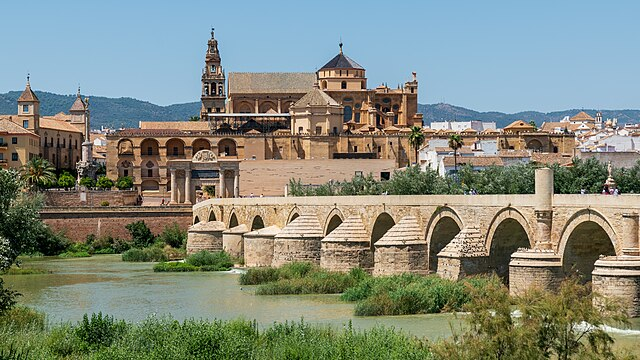
\includegraphics[keepaspectratio]{img/puente.jpg}}

}

\caption{Esto es una foto de un puente enlazada con una web y con texto
alternativo y una descripción como pop-up}

\end{figure}%

\newpage{}

\subsection{Varias imágenes unidas}\label{varias-imuxe1genes-unidas}

\begin{figure}

\begin{minipage}{0.33\linewidth}

\begin{figure}[H]

{\centering 
\includegraphics[width=\linewidth,height=3.125in,keepaspectratio]{tree_01.png}

}

\subcaption{Especie A}

\end{figure}%

\end{minipage}%
%
\begin{minipage}{0.33\linewidth}

\begin{figure}[H]

{\centering 
\includegraphics[width=\linewidth,height=3.125in,keepaspectratio]{tree_02.png}

}

\subcaption{Especie B}

\end{figure}%

\end{minipage}%
%
\begin{minipage}{0.33\linewidth}

\begin{figure}[H]

{\centering 
\includegraphics[width=\linewidth,height=3.125in,keepaspectratio]{tree_03.png}

}

\subcaption{Especie C}

\end{figure}%

\end{minipage}%

\end{figure}%

Al escribir:

\begin{verbatim}
::: {layout="[30,30,30]" layout-valign="bottom"}
![Especie A](tree_01.png){height=300}

![Especie B](tree_02.png){height=300}

![Especie C](tree_03.png){height=300}
:::
\end{verbatim}

\newpage{}

\subsection{Incluir imágenes con ayuda de
knitr}\label{incluir-imuxe1genes-con-ayuda-de-knitr}

Se hace con ayuda de código R y la función:
\texttt{knitr::include\_graphics()}.

\begin{figure}[H]

\centering{


\includegraphics[width=0.5\linewidth,height=\textheight,keepaspectratio]{tree_03.png}

}

\caption{\label{fig-arbol03knitr}Imagen de un árbol}

\end{figure}%

El código utilizado ha sido:

\begin{figure}[H]

\centering{


\includegraphics[width=0.5\linewidth,height=\textheight,keepaspectratio]{tree_03.png}

}

\caption{\label{fig-arbol03knitr2}Imagen de un árbol}

\end{figure}%




\end{document}
